\graphicspath{ {./JiaweiZhuang/HW2_figures/different_width/} }

\begin{solution} 

Running the simulation with varying sizes of $w=10, 20, 30, 40, 50$, we obtain the following velocity profiles. The steady state velocity $u$ is shown in Fig \ref{fig:ux_ws_case1} and Fig \ref{fig:ux_ws_case2}. The periodic cases has parabola-like velocity profile at the boundary, while the non-periodic we imposed to have uniform profile over $y$ near boundary.

\begin{figure}[H]
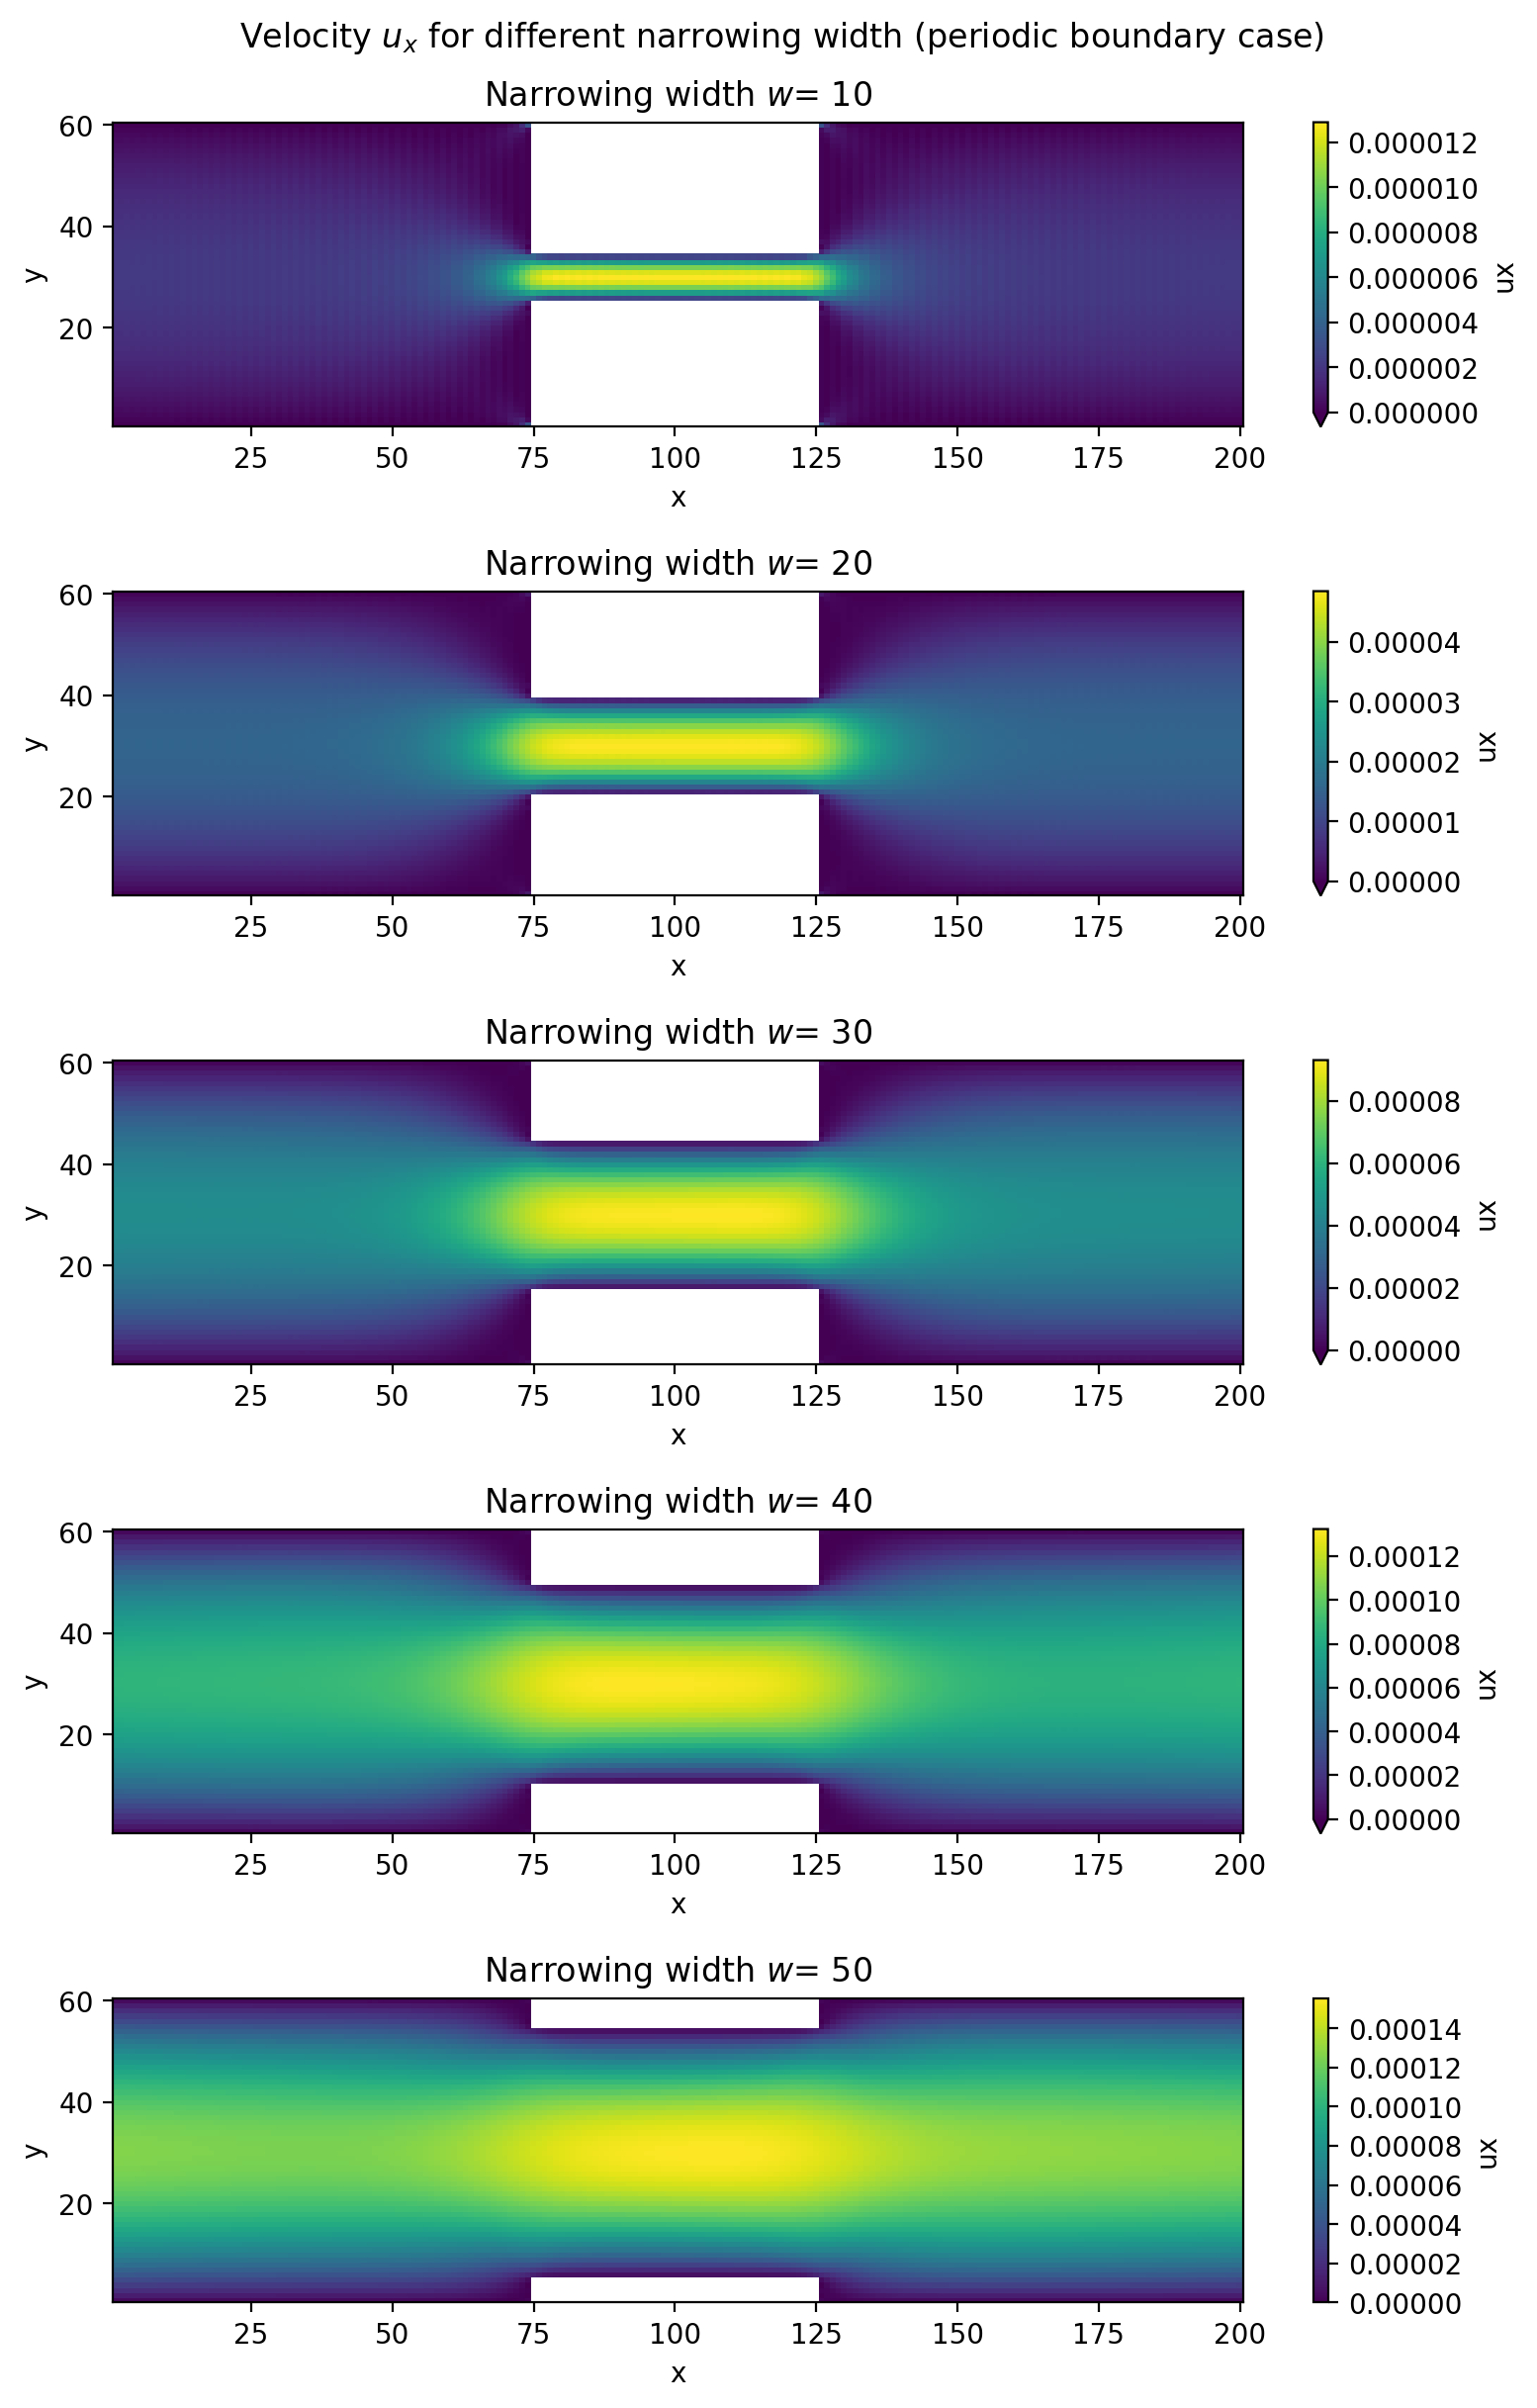
\includegraphics[scale=0.6]{case1_ux_different_width}
\centering
\caption{Velocity field with different narrowing width, for periodic boundary case.}
\label{fig:ux_ws_case1}
\end{figure}

\end{solution}

\begin{solution} 

\begin{figure}[H]
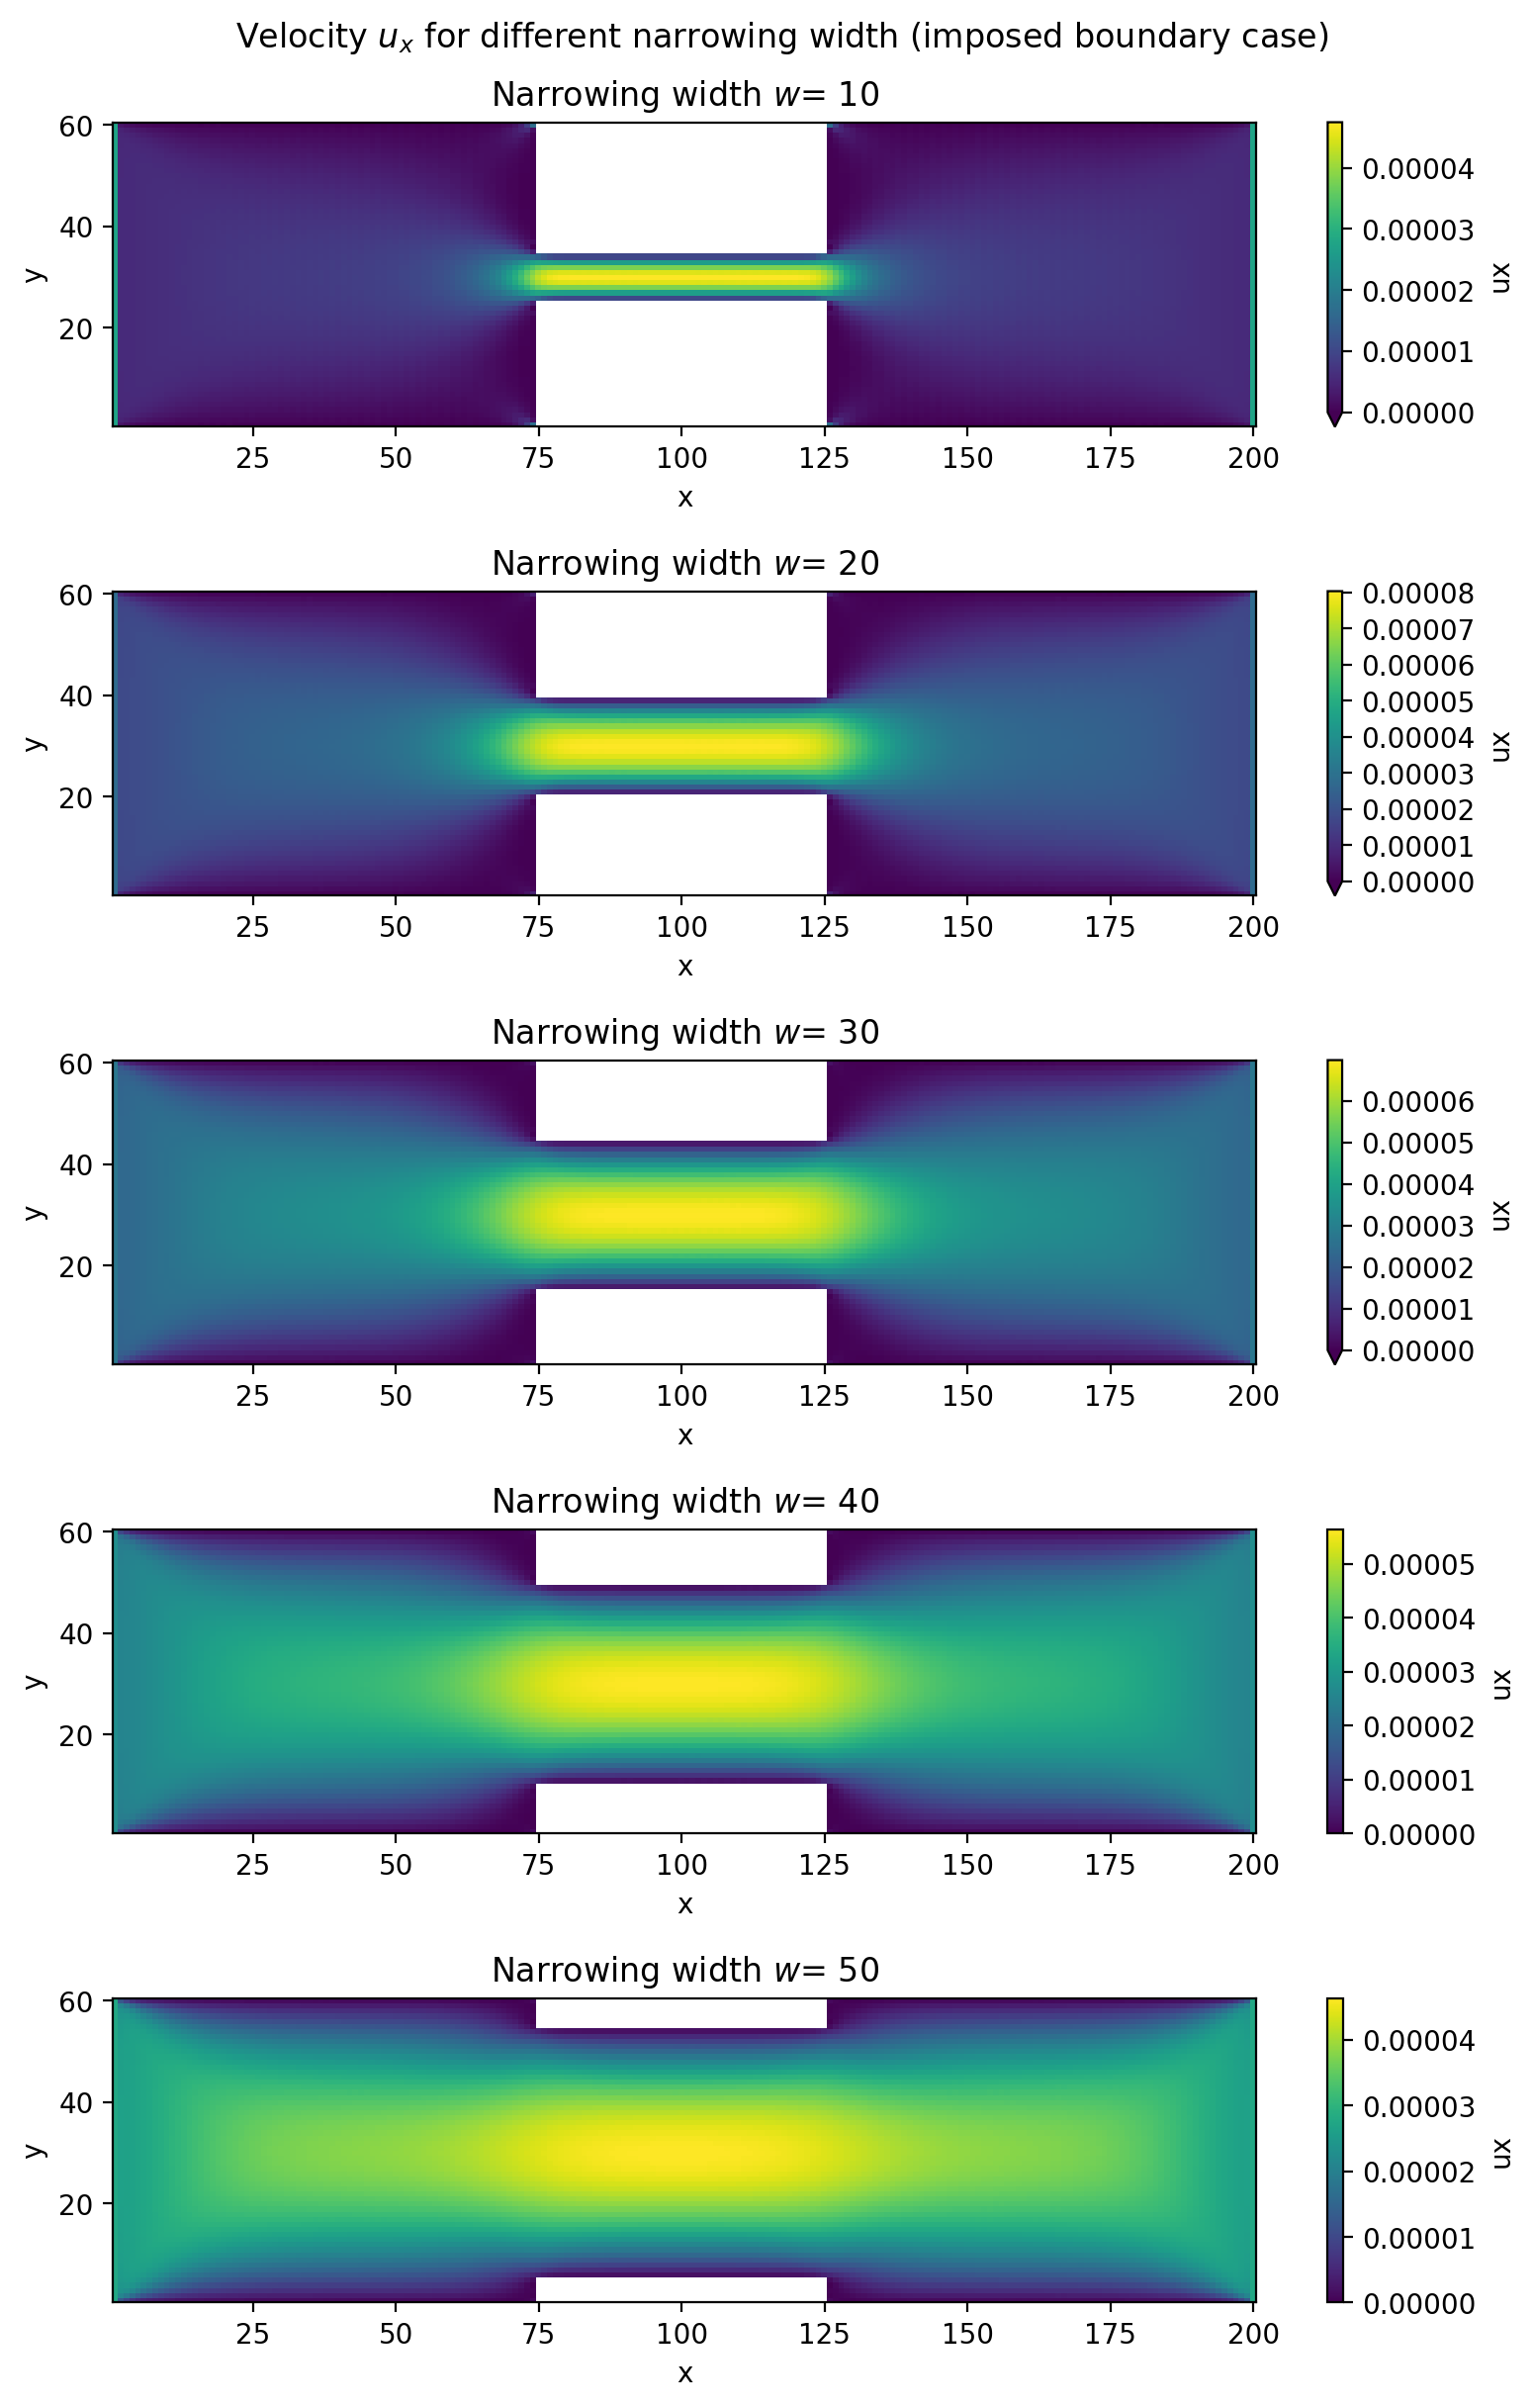
\includegraphics[scale=0.6]{case2_ux_different_width}
\centering
\caption{Velocity field with different narrowing width, for non-periodic boundary case.}
\label{fig:ux_ws_case2}
\end{figure}

\end{solution}


\begin{solution} 

We then compute the volume flow rate by integrating over $y$ and then averaging over $x$. The rates for different $w$ are shown in Fig \ref{fig:flow_ws_case1} and Fig \ref{fig:flow_ws_case2}. In both cases, the rate increases with the channel width, as expected.

\begin{figure}[H]
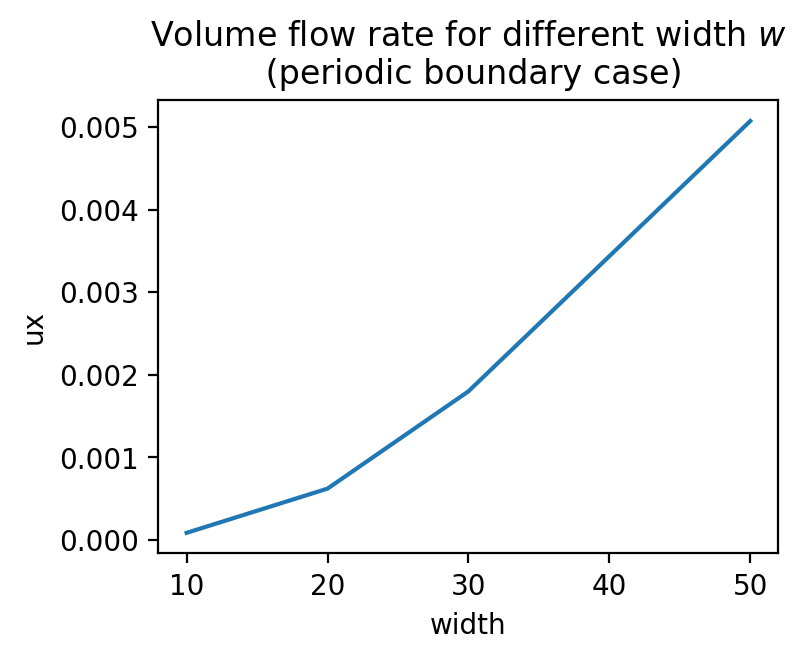
\includegraphics[scale=0.6]{case1_ws_volume_flow}
\centering
\caption{Volume flow rate (averaged) with different narrowing width, for periodic boundary case.}
\label{fig:flow_ws_case1}
\end{figure}

\begin{figure}[H]
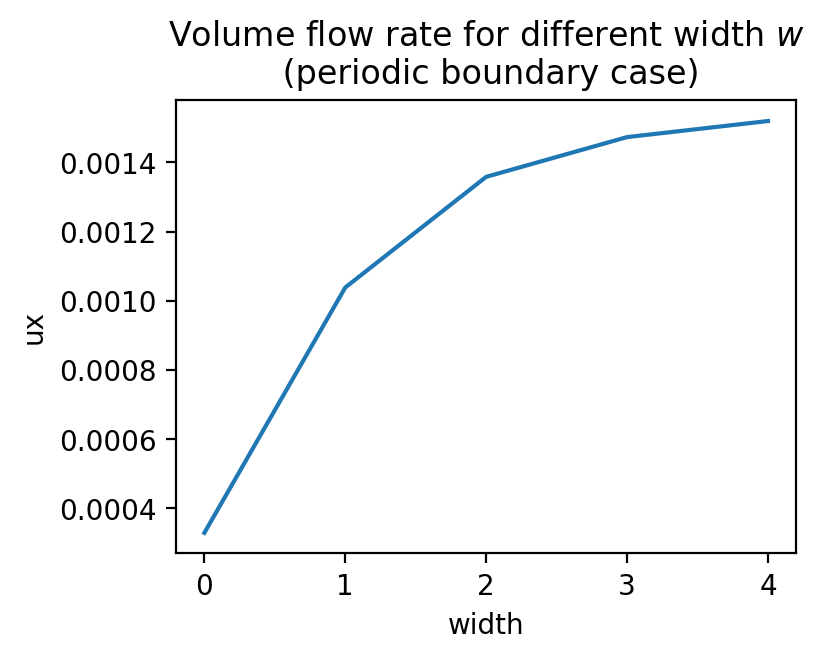
\includegraphics[scale=0.6]{case2_ws_volume_flow}
\centering
\caption{Volume flow rate (averaged) with different narrowing width, for non-periodic boundary case.}
\label{fig:flow_ws_case2}
\end{figure}

\end{solution}